\documentclass[Protokollheft.tex]{subfiles}
\begin{document}
\chapter{Grundlagen der Methode der Finiten Integration 2}
%--------------- Start Vorbereitungsaufgaben ---------------

\section{Vorbereitungsaufgaben}

% --> Aufgabe
\begin{framed}
	\noindent \textbf{1.} Überlegen Sie sich, wie man ausgehend vom 3-fach Index $i,j,k$ (vgl. Gl.~(3.1)) die Randpunkte eines kartesischen Rechengebietes im kanonischen Indizierungsschema bestimmt (eine Skizze ist hilfreich). Schreiben Sie hierfür ein Schleifenkonstrukt in Pseudocode.\label{exer:boundIdx}
\end{framed}


Ausgehend von einem 3-fach Index i,j,k lasen sich die Randpunkte eines Kartesischen Rechengitters im kanonischen Indizierungsschema durch ablaufen der Außenseiten bestimmen. Hierbei werden nacheinander i,j und k zu Null gesetzt und die beiden anderen Variablen Variiert. Anschließend wird selbiges mit einem Festsetzen beim Maximalwert der jeweiligen Variable wiederholt. Alle hierbei erreichten Punkte liegen auf den Außenseiten des Gitters. 
\noindent
Im Pseudocode lässt sich diese Verfahren für eine Richtung $i$ darstellen durch

\begin{algorithmic}[1]
	\STATE $c \leftarrow 1$
	\STATE $d \leftarrow 1$
	\WHILE{ c <= jmax} 
	\WHILE{ d <= kmax}
		\STATE $AddToListBoundaryElementAt(1,c,d)$
		\STATE $d \leftarrow d+1$
	\ENDWHILE
	
	\STATE $c \leftarrow c+1$
	\ENDWHILE
	
	\STATE $c \leftarrow 1$
	\STATE $d \leftarrow 1$
	\WHILE{ c <= jmax} 
	\WHILE{ d <= kmax}
	\STATE $AddToListBoundaryElementAt(i_{max},c,d)$
	\STATE $d \leftarrow d+1$
	\ENDWHILE	
	\STATE	$c \leftarrow c+1$
	\ENDWHILE
	
\end{algorithmic}
\noindent
Die Funktion $AddToListBoundaryElementAt$ führt eine Liste mit den kanonischen Indizes, welche unter Zuhilfenahme von $M_x,\ M_y$ und $M_z$ bestimmt werden, der Randpunkte.  

% --> Aufgabe
\begin{framed}
	\noindent \textbf{2.} Wie sehen für ein äquidistantes, kartesisches Gitter die Geometriematrizen $\DS$, $\DSd$, $\DA$ und $\DAd$ aus? Was ist bei den Rändern zu beachten? Welche Dimensionen besitzen die Matrizen?\label{exer:geoMatsStructure}
\end{framed}
\noindent
Für eine äquidistantes, kartesisches Gitter bildet die Matrix $DS$ eine Diagonalmatrizen mit dem Abstand $\Delta x$ auf der Diagonalen. Die duale Matrix $\DSd$ unterscheidet sich hiervon nur dadurch, das die Randelemente mit ½ multipliziert werden. \\
Für die Flächenzentrierten $\DA$ gilt simultan das sie Diagonalmatrizen mit den Flächeninhalt $\Delta x^2$ sind. Bei der Dualen Flächenmatrix $\DAd$ muss nun bei den Randelementen allerdings unterschieden werden zwischen denen die an einer Kante liegen und mit ½ multipliziert werden und denen an einer Ecke die mit ¼ multipliziert werden. \\
Falls hier bereits Geisterkanten entfernt worden sind, sind bei den primären Matrizen $\DS$ und $\DA$ die Geisterelemente jeweils Null. \\
\noindent
Die Matrizen besitzen immer die Dimension  $[np,\ 3np]$ mit $np$ als Anzahl der Gitterpunkte.

% --> Aufgabe
\begin{framed}
	\noindent \textbf{3.} Skizzieren Sie kurz, wie sich die Materialmatrizen zusammenstellen. Wie sind hierbei die Randbedingungen (elektrisch \& magnetisch) einzuarbeiten bzw. muss überhaupt eine Änderung vorgenommen werden?\label{exer:materialMats}
\end{framed}
\noindent
Skizze:\\
$$\Meps =\DAd\Deps\DS^{-1} = \begin{bmatrix}
\tilde{dA}(1) & & \\
& \ddots & \\
& & \tilde{dA}(3\cdot\mathrm{np})
\end{bmatrix}
\cdot
 \begin{bmatrix}
\varepsilon(1) & & \\
& \ddots & \\
& & \varepsilon(3\cdot\mathrm{np})
\end{bmatrix}
\cdot
\begin{bmatrix}
\mathrm{ds}(1) & & \\
& \ddots & \\
& & \mathrm{ds}(3\cdot\mathrm{np})
\end{bmatrix}^{-1}$$
$$\Mmui=\DSd\Dmui\DA^{-1}=
\begin{bmatrix}
\tilde{ds}(1) & & \\
& \ddots & \\
& & \tilde{ds}(3\cdot\mathrm{np})
\end{bmatrix}
\cdot
 \begin{bmatrix}
\mu^{-1}(1) & & \\
& \ddots & \\
& & \mu^{-1}(3\cdot\mathrm{np})
\end{bmatrix}
\cdot
\begin{bmatrix}
\mathrm{dA}(1) & & \\
& \ddots & \\
& & \mathrm{dA}(3\cdot\mathrm{np})
\end{bmatrix}^{-1}$$
\noindent
Wenn man elektrische Randbedingung hat, muss man die tangentiale Komponente der Permitivität und normale Komponente der Permeabilität am Rand auf Null setzen. Bei magnetischer Randbedingung ist die tangentiale Komponente der magnetischen Feldstärke und normale Komponente des elektrischen Feldes gleich Null. Bei den Materialmatrizen gibt es keine Veränderungen. Die normale Komponente auf dem primären Gitter ist eine Geisterkante und für die Geisterkante ist keine Kante auf dem dualen Gitter definiert. Der Code dazu ist in Listing \ref{lst:mgn_RB} zu sehen.
\begin{lstlisting}[caption={Einsetzten der elektrischen Randbedigungen},label={lst:mgn_RB}]
%% Randbedingungen

% Spezialfall nur bei PEC Rand (bc=1)
if bc==1
 for i=1:nx
  for j=1:ny
   for k=1:nz
    n=1+(i-1)*Mx+(j-1)*My+(k-1)*Mz;
    if k==1 || k==nz
     meanEpsX(n)=0; 
     meanEpsY(n)=0;
    endif
    if j==1 || j==ny
     meanEpsX(n)=0; 
     meanEpsZ(n)=0;
    endif
    if i==1 || i==nx
     meanEpsZ(n)=0; 
     meanEpsY(n)=0;
    endif
   end
  end
 end
end
\end{lstlisting}



% --> Aufgabe
\begin{framed}
	\noindent \textbf{4.} Um die im Versuch zu implementierende Visualisierung zu testen, soll ein vorgegebenes
    rotationssymmetrisches Feld in Zylinderkoordinaten nach der analytischen Formel
    \begin{align}
     \vec{D}(r,\varphi,z)=\frac{1}{r^2} \er
    \end{align}
    visualisiert werden. Es soll ein äquidistantes Gitter benutzt werden, dessen Mitte genau dem Koordinatenursprung entspricht.\\
Bestimmen Sie die diskreten Größen $\dfitloc(n)$ und $\efitloc(n)$ des vorgegebenen Feldes. Zur Vereinfachung soll bei der hierfür notwendigen Integration der Feldwert in der Mitte der Strecke bzw. Fläche als repräsentativ gelten und damit als konstant über dem gesamten Element angenommen werden. \\
    \ \\
    {\textbf{Hinweis:}} Transformieren Sie zuerst zur Bestimmung der notwendigen Feldwerte das gegebene Feld in kartesische Koordinaten $\vec{D}(x,y,z)$.\label{exer:visualizeFieldPrep}
%
\end{framed}
\noindent
Transformiert man $\vec{D}(r,\varphi,z)$ in kartesische Koordinaten ergibt sich
\begin{equation*}
	\vec{D}(x,y,z)=\frac{x}{(x^2+y^2)^{\frac{3}{2}}} \ \vec{e}_x+\frac{y}{(x^2+y^2)^{\frac{3}{2}}} \vec{e}_y.
\end{equation*}
Möchte man nun $\dfitloc(n)$ berechnen muss man einfach $\vec{D}$ am Mittelpunkt der dualen Fläche auswerten und mit dem Flächeninhalt multiplizieren. Um daraus \efitloc(n) zu bestimmt muss einfach die Material Matrix $\Meps$ mit \dfitloc(n) multipliziert werden. Daraus folgt:
\begin{eqnarray*}
\dfitloc(n)&=&\vec{D}(x_n,y_n,z_n)\ \tilde{dA}\\
\efitloc(n)&=&\Meps\dfitloc
\end{eqnarray*}



\section{Aufgaben während der Praktikumssitzung}

\subsection{Materialmatrizen}

% --> Aufgabe
\begin{framed}
	\noindent \textbf{1.} Zuerst sollen zwei Funktionen zum Bestimmen der Geometriematrizen $\DS$, $\DSd$ und $\DA$ geschrieben werden:
\begin{align}
\lstinline{[DS, DSt]} &= \lstinline{createDS(msh)} \label{pro:createDs}\\
\lstinline{[DA]} &= \lstinline{createDA(DS)} \label{pro:createDA}
\end{align}
Wie kann mit der zweiten Funktion auch $\DAd$ bestimmt werden?\label{exer:createDS_DA}
\end{framed}

Analog zu $\DA$ kann man zweite Funktion verwenden um $\DAd$ bestimmen. Man soll nur als Eingabe Parameter $\DSd$ setzen.
\begin{align*}
	\lstinline{[DS, DSt]} &= \lstinline{createDS(msh)} \\
	\lstinline{[DAt]} &= \lstinline{createDA(DSt)} 
\end{align*}
% --> Aufgabe
\begin{framed}
	\noindent \textbf{2.} Nun sollen die Funktionen
\begin{align}
\lstinline{[Deps]} &= \lstinline{createDeps(msh, DA, DAt, eps_r, bc)} \label{pro:createDeps}\\
\lstinline{[Meps]} &= \lstinline{createMeps(DAt, Deps, DS)} \label{pro:createMeps}
\end{align}
geschrieben werden, um die $\Meps$-Matrix \lstinline{Meps} aus der $\Deps$-Matrix \lstinline{Deps}
der gemittelten Permittivitäten zu bestimmen.
\lstinline{bc} $=1$ soll dabei elektrische und \lstinline{bc} $=2$ magnetische Randbedingungen bedeuten.
Die Materialverteilung auf dem Gitter \lstinline{msh} soll inhomogen und isotrop bezüglich der Raumrichtungen sein. Zur besseren Übersicht sollen bei der Übergabe relative Permittivitäten verwendet werden. \lstinline{eps_r} soll damit als $N_\text{P}\times 1$ Matrix übergeben werden, also für jedes der $N_\text{P}$ primären Volumen ein $\eps_\text{r}$-Wert.
\\
\textbf{Hinweis:} Für das Invertieren von $\DS$ ist die Methode
\lstinline{nullInv} vorgegeben.\label{exer:createDeps_Meps}
\end{framed}



% --> Aufgabe
\begin{framed}
	\noindent \textbf{3.} Die Funktion~\eqref{pro:createMeps} soll nun mit den Parametern
\lstinline{xmesh = [-2 0 2]}, \lstinline{ymesh = [-1 0 1]}, \lstinline{zmesh = [0 1]} und
isotropem $\eps=\eps_0$ die Materialmatrix
$\Meps$ für elektrische Randbedingungen berechnen und ausgeben. Vervollständigen Sie hierfür das bereits gegebene Skript \lstinline{exampleMeps.m}\label{exer:MepsExample}
\end{framed}



\subsection{Interpolation und Visualisierung}

% --> Aufgabe
\begin{framed}
	\noindent \textbf{4.} Programmieren Sie eine Routine
\begin{align}
	\lstinline{eField = fitInt(msh, eBow)} \; , \label{mthd:fitInt}
\end{align}	
die die Komponenten von $\efit$ als $\vec{E}$-Feld auf die primären Punkte interpoliert.\label{exer:fitInt}
\end{framed}



% --> Aufgabe
\begin{framed}
	\noindent \textbf{5.} Schreiben sie eine Methode
\begin{align}
	\lstinline{plotEBow(msh, eBow, indz)} \; , \label{mthd:plotEBow}
\end{align}
die auf Methode~\eqref{mthd:fitInt} aufbauend $\efit$ interpoliert und den
Betrag des $\vec{E}$-Feldes mit dem \matlab-Befehl \lstinline{surf} in einer
$x$-$y$-Ebene mit Index \lstinline{indz} grafisch darstellt. Verwenden Sie hierfür bitte elektrische Randbedingungen.
\\
\textbf{Hinweis:} Nutzen Sie auch für das Invertieren von $\Meps$ die vorgegebene Methode
\lstinline{nullInv}.\label{exer:plotEBow}
\end{framed}



% --> Aufgabe
\begin{framed}
	\noindent \textbf{6.} Geben Sie das rotationssymmetrische Feld aus der Vorbereitung als
Vektor $\dfit$ vor, berechnen Sie daraus mit Hilfe der Materialmatrix $\Mepsi$
das Feld $\efit$ und wenden Sie dann Methode \eqref{mthd:plotEBow} an. Visualisieren Sie außerdem die selbe Schnittebene mit der in Versuch 2 vorgestellten Methode \lstinline{plotEdgeVoltage}. Vervollständigen Sie hierfür den ersten Teil des bereits gegebenen Skripts \lstinline{exampleVisualEfield.m}\label{exer:exampleVisualEfield1}
\end{framed}
\noindent
Das elektrische Feld für isotrope Materialien ist in den Abbildungen \ref{Abb:61} und \ref{Abb:62} dargestellt.

% --> Aufgabe
\begin{framed}
	\noindent \textbf{7.} Überlegen Sie sich, welche Änderungen an den bisher implementierten Methoden 
vorgenommen werden müssen, um ein anisotropes Material zu verwenden. Ändern Sie 
Ihre Implementierung entsprechend und verwenden Sie ein anisotropes Material mit unterschiedlichen
Permittivitäten in $x$- und $y$-Richtung (z.\,B.
$\eps_x / \eps_y=4$) sowie elektrische
Randbedingungen. Interpolieren und visualisieren Sie das Feld
$\efit$ wie in der Aufgabe zuvor. Visualisieren Sie auch hier das Ergebnis zusätzlich mit der Methode \lstinline{plotEdgeVoltage}. Vervollständigen Sie hierfür den zweiten Teil des bereits gegebenen Skripts \lstinline{exampleVisualEfield.m}\label{exer:exampleVisualEfield2}\\
\end{framed}
\noindent
Das elektrische Feld für anisotrope Materialien ist in den Abbildungen \ref{Abb:71} und \ref{Abb:72} dargestellt.

\section{Fragen zur Ausarbeitung}

% --> Aufgabe
	\begin{framed}
	\noindent \textbf{1.} Erstellen Sie eine 2D-Skizze einer dualen
	Gitterfläche mit den zugehörigen primären Gitterzellen, welche
    zur Mittelung der Permittivität notwendig sind (siehe (3.10)).\label{exer:averagingEps}
\end{framed}
\noindent
Die duale Fläche mit den zugehörigen primären Gitterzellen sind in Abbildung \ref{Abb:A1} zu sehen.


% --> Aufgabe
	\begin{framed}
	\noindent \textbf{2.} Häufig werden für die Visualisierung der magnetischen Feldstärke
	$\Hv$ die entsprechenden Komponenten ebenfalls auf den Punkten des
	primären Gitters gemittelt und nicht auf den dualen
	Punkten. Beschreiben Sie für diese Mittelung \emph{kurz} eine geeignete Vorgehensweise (kleine Skizze sinnvoll)
	und gehen Sie dabei auch auf die Randbedingungen ein.\label{exer:averageHfield}
\end{framed}
\noindent
Für die Mittelung von $\Hv$ auf den Primären Punkten muss zunächst die magnetische Flussdichte $\vec{B}$ von den 4 anliegenden primären Flächen mit $\bar{B}=\frac{1}{4}(B_1+B_2+B_3+B_4)$ gemittelt werden. Nun muss man weiterhin die Materialkonstate $\mu$ über die 4 anliegenden  Flächen mit $\bar{\mu}=\frac{1}{4}(\mu_1+\mu_2+\mu_3+\mu_4)$ mitteln. Die Feldstärke $\Hv$ ergibt sich nun aus der Materialbeziehung zwischen $\vec{B}$ und $\Hv$. Damit erhalten wir $\Hv=\bar{\mu}\bar{B}$. 

\section{Fazit}
Wie in der Ausarbeitung deutlich wird, ist es nun möglich Materialmatrizen zu erstellen, sowie elektrische Felder zu visualisieren.

\section{Abbildungen}
\begin{figure}[h!]
	\centering
	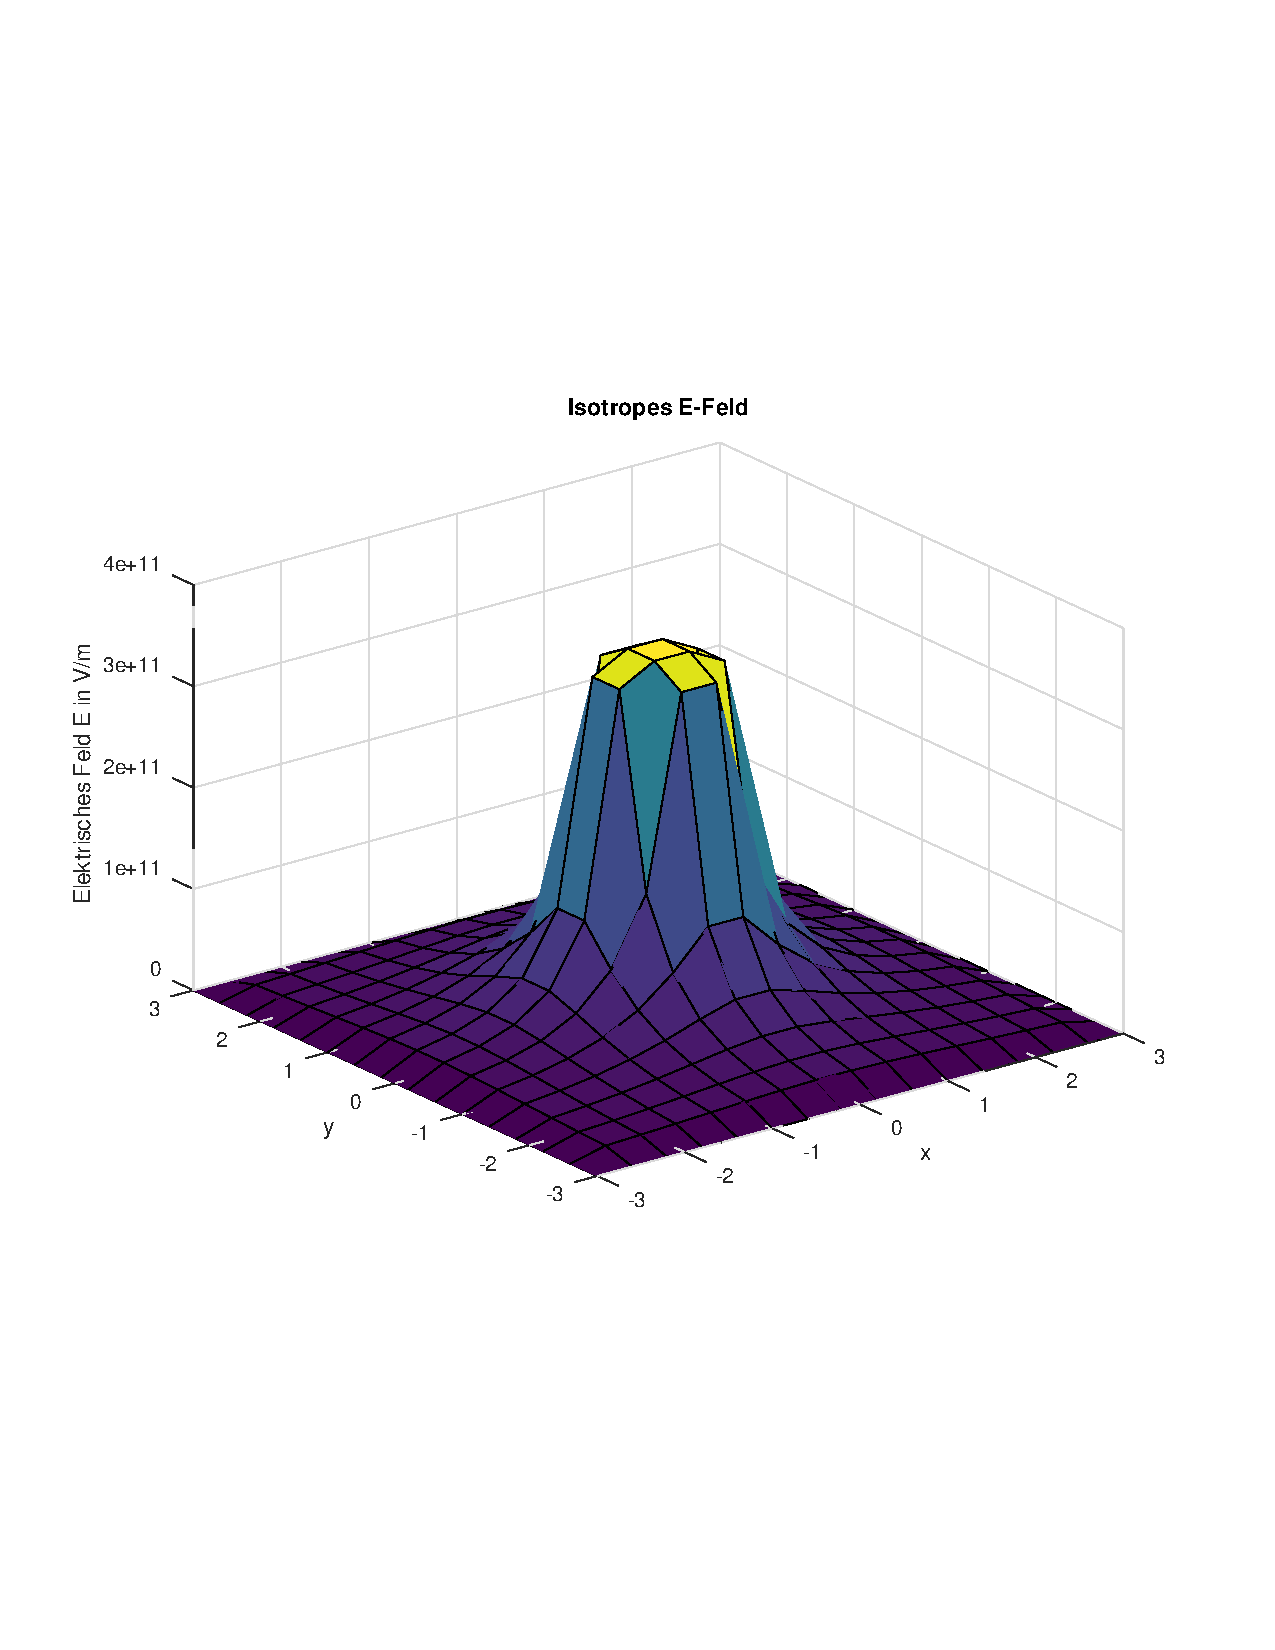
\includegraphics[trim = 10mm 60mm 10mm 50mm, clip, width=0.7\textwidth]{efield_1.pdf}
	\caption{Elektrisches Feld bei isotroper Materialverteilung in 3D.}
	\label{Abb:61}
\end{figure}

\begin{figure}[h!]
	\centering
	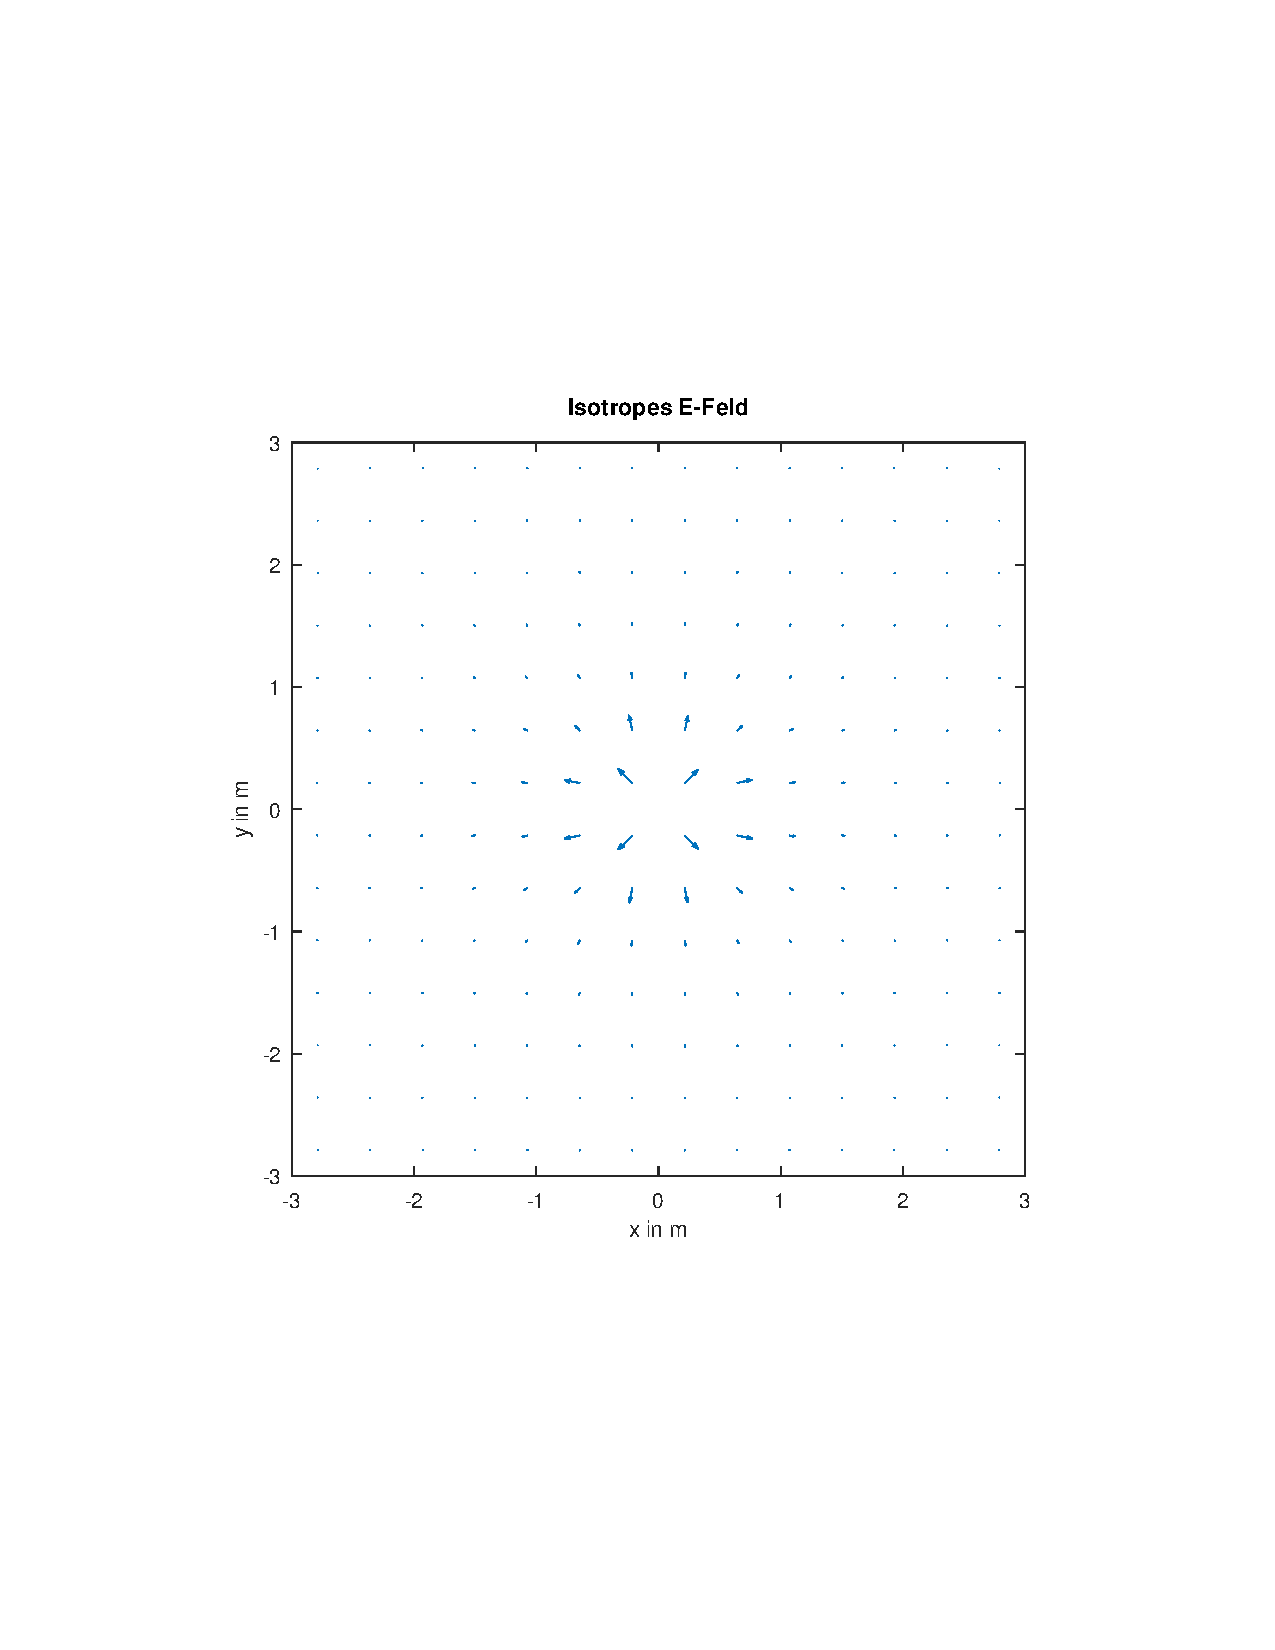
\includegraphics[trim = 10mm 60mm 10mm 50mm, clip, width=0.7\textwidth]{efield_2.pdf}
	\caption{Elektrisches Feld bei isotroper Materialverteilung dargestellt mit Vektorpfeilen.}
	\label{Abb:62}
\end{figure}
\begin{figure}[h!]
	\centering
	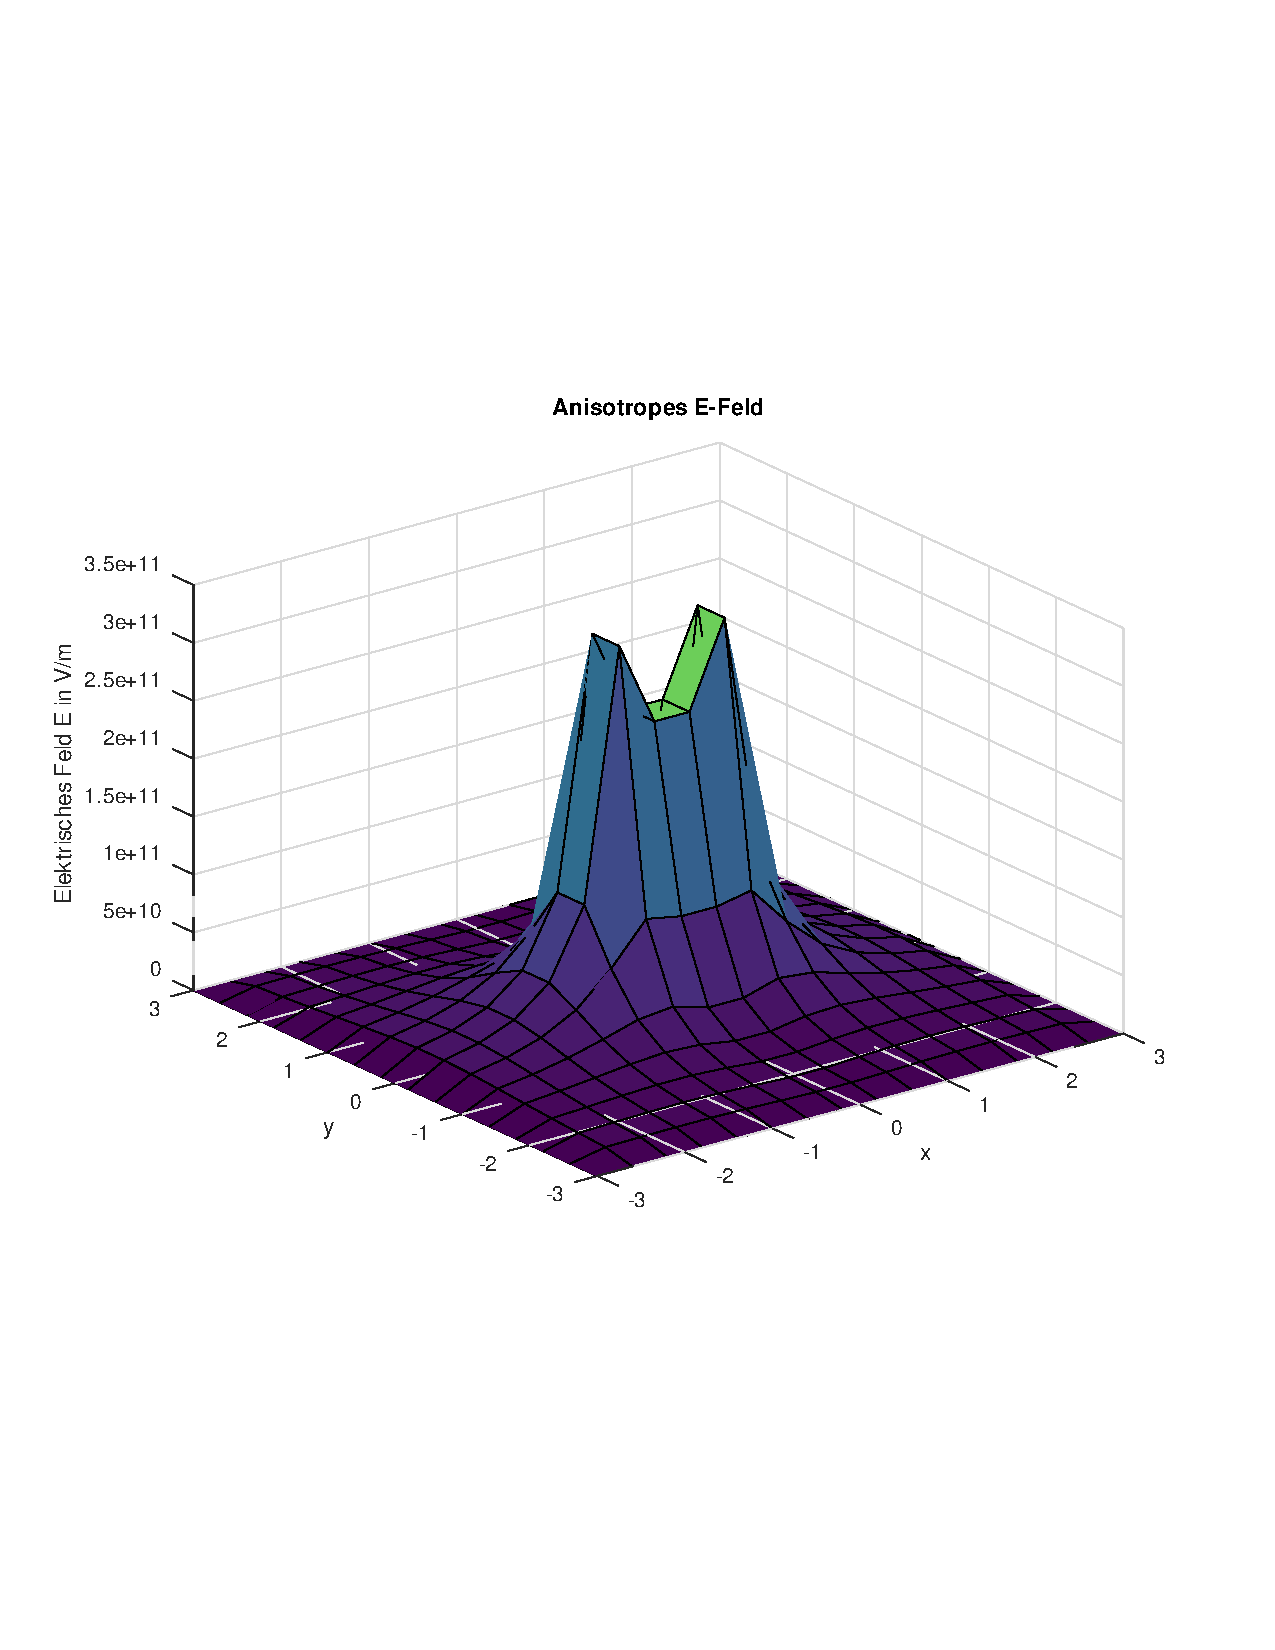
\includegraphics[trim = 10mm 60mm 10mm 50mm, clip, width=0.7\textwidth]{efield_3.pdf}
	\caption{Elektrisches Feld bei anisotroper Materialverteilung in 3D.}
	\label{Abb:71}
\end{figure}

\begin{figure}[h!]
	\centering
	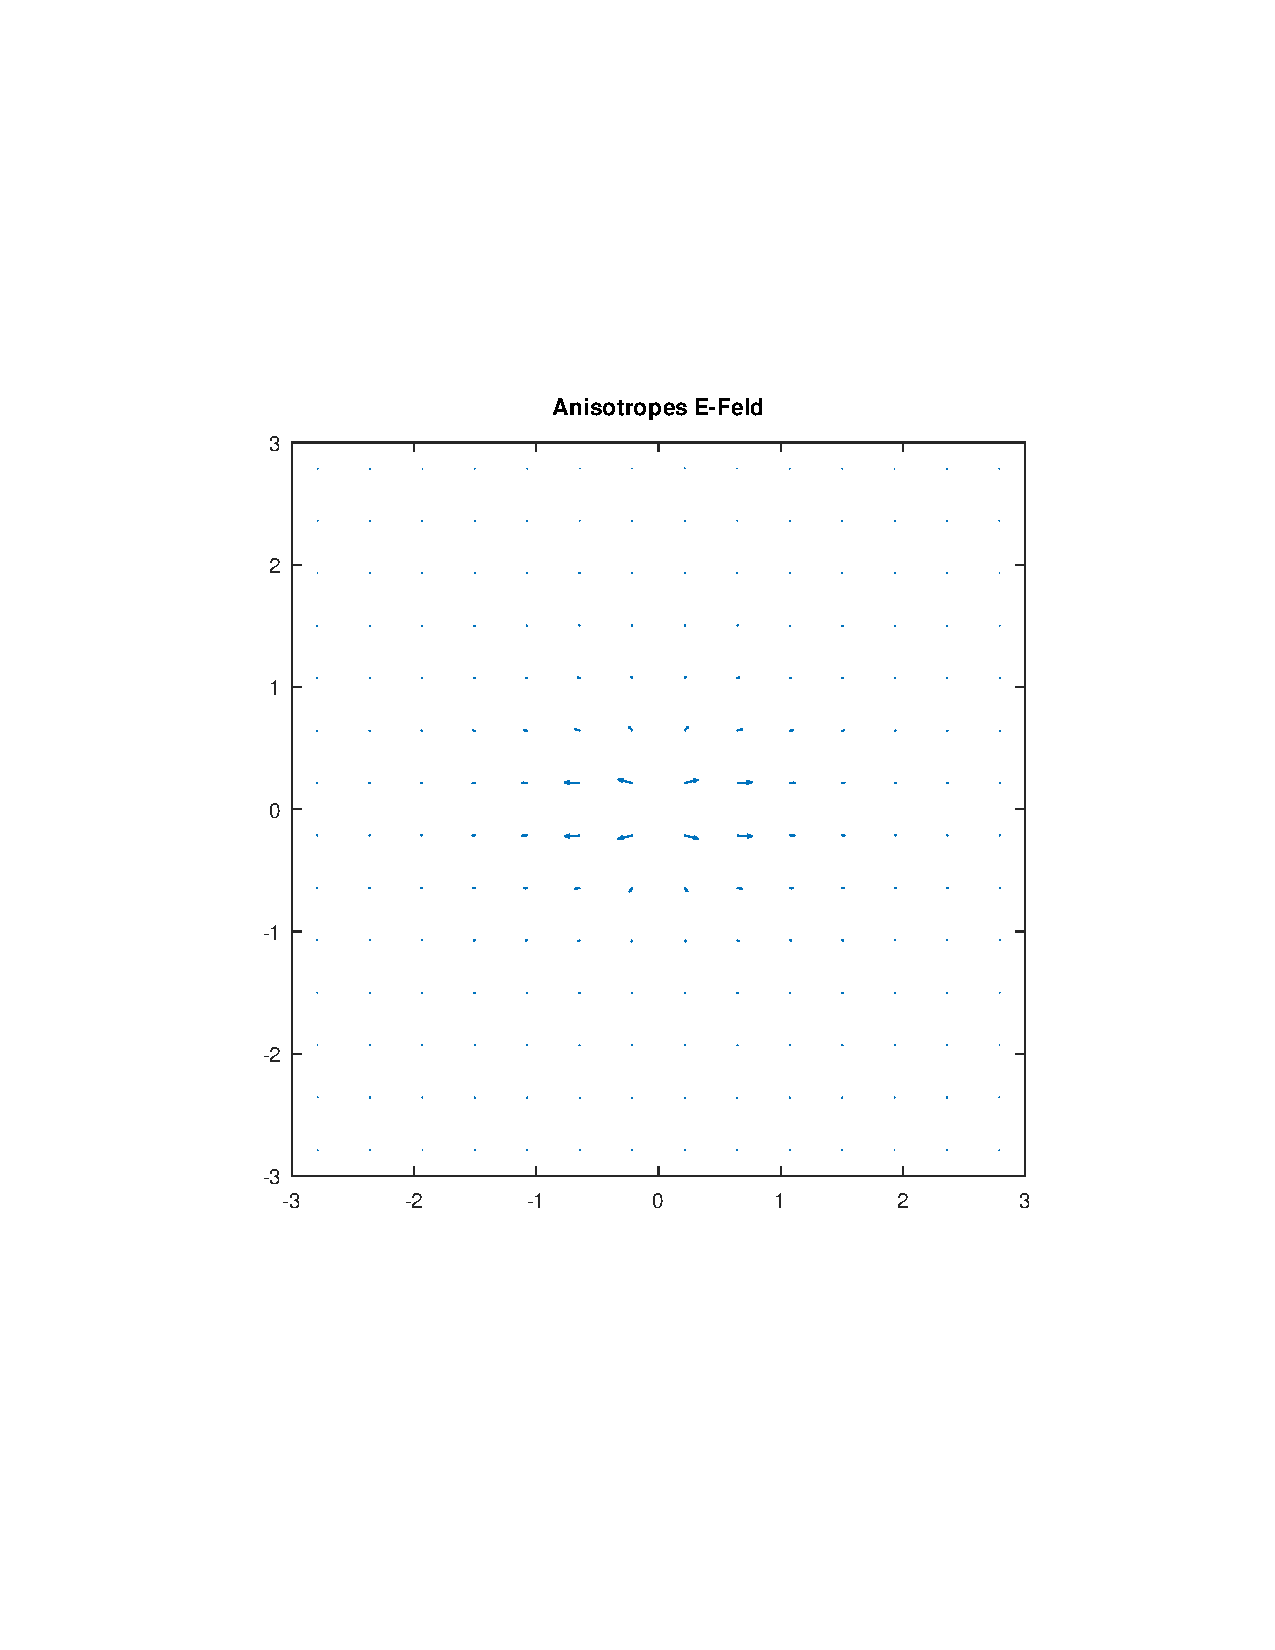
\includegraphics[trim = 10mm 60mm 10mm 50mm, clip, width=0.7\textwidth]{efield_4.pdf}
	\caption{Elektrisches Feld bei anisotroper Materialverteilung dargestellt mit Vektorpfeilen.}
	\label{Abb:72}
\end{figure}
\begin{figure}[h!]
	\centering
	
\includegraphics[trim = 0mm 0mm 0mm 0mm, clip, width=0.5\textwidth]{Ausarbeitung1.png}
	\caption{Duale Fläche (Mitte) mit den primären Gitterzellen. Die für die Mittelung interessanten Bereiche sind schraffiert.}
	\label{Abb:A1}
\end{figure}
\begin{figure}[h!]
	\centering
	
\includegraphics[trim = 0mm 0mm 0mm 0mm, clip, width=0.5\textwidth]{Ausarbeitung2.png}
	\caption{Darstellung der örtlichen Beziehungen zwischen $\Hv$ und $\vec{B}$.}
	\label{Abb:A1}
\end{figure}

\end{document}
